\newpage
\pagestyle{empty}

\begin{minipage}[c]{.25\linewidth}
	
\includegraphics[width=4cm]{images/Logo-LEnsE.png}
\end{minipage} \hfill
\begin{minipage}[c]{.4\linewidth}

\begin{center}
\vspace{0.3cm}
{\Large \textsc{Opto-Electronique}}

\medskip

\textbf{\Large Ressources}

\end{center}
\end{minipage}\hfill

\vspace{0.5cm}

\noindent \rule{\linewidth}{1pt}
\section{Tracer la réponse indicielle d'un système linéaire}
\label{ressource:RepIndic}


%%%%%%%%%%%%%%%%%%%%

La réponse indicielle fournit des informations essentielles sur les \textbf{caractéristiques dynamiques} d'un système. Elle permet d'analyser le comportement transitoire et le comportement à l'état stable d'un système. Par exemple, on peut observer le temps de montée, le temps de stabilisation, le dépassement (ordre supérieur à 2), et l'erreur en régime permanent.

Elle est aussi appelée \textbf{réponse à un échelon} unitaire. Elle correspond à la sortie d'un système lorsqu'un signal de type échelon est appliqué en entrée. Un \textbf{échelon unitaire} est une fonction qui passe de 0 à 1 à un instant donné, généralement considéré à $t = 0$. 

La figure~\ref{fig:ordre2} est une capture d'écran d'oscilloscope représentant la réponse indicielle d'un système passe-bas du second ordre. 

\begin{figure}[h!]
    \centering
	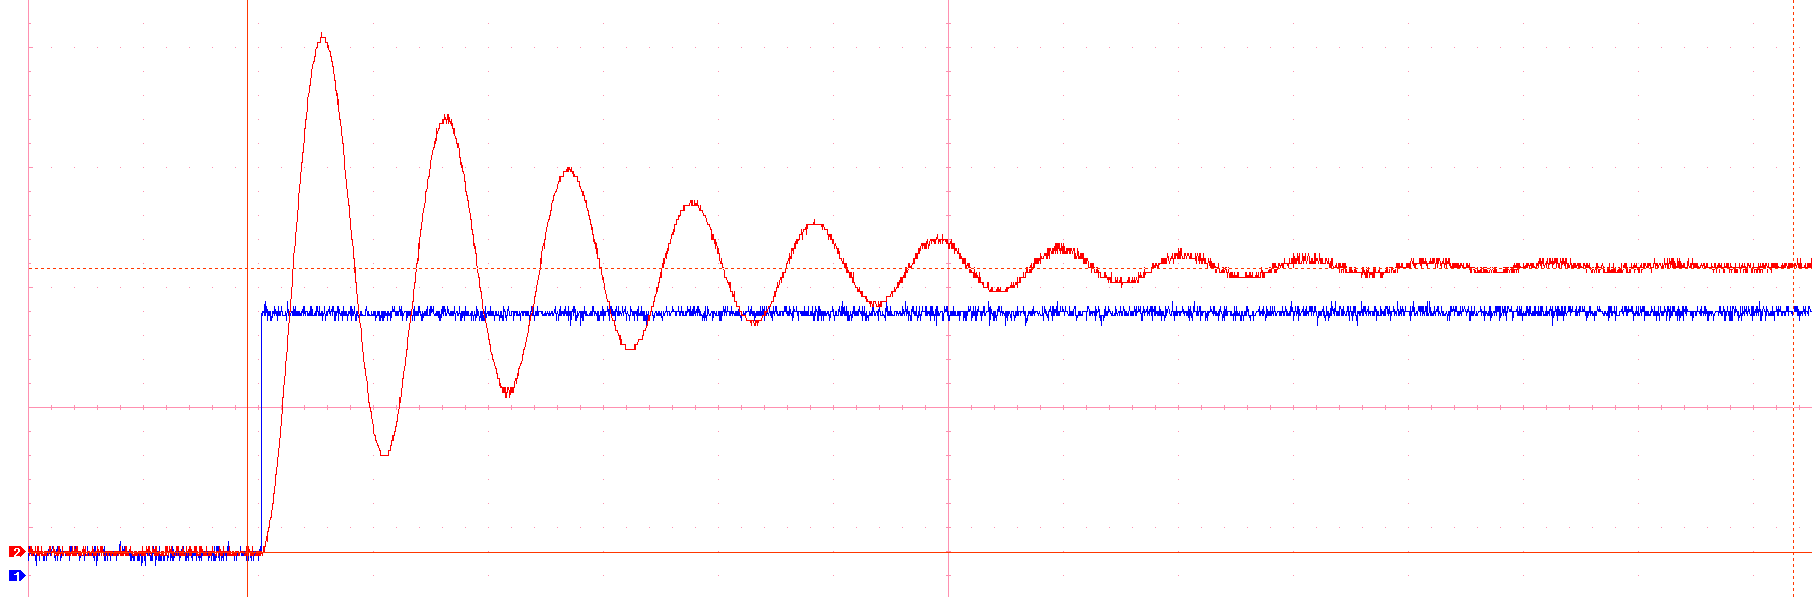
\includegraphics[width=0.9\textwidth]{images/ri_ordre2.png}
	
    \caption{Capture d'écran d'oscilloscope d'un échelon de tension $V_E$ (en bleu) appliqué à un système de type passe-bas d'ordre 2 avec résonance. La tension de sortie $V_S$ (en rouge) représente la réponse indicielle de ce système. Le calibre vertical est de 1V/carreau pour $V_E$ et de 2V/carreau pour $V_S$. L'échelle horizontale est de 1ms/carreau.}
    \label{fig:ordre2}
\end{figure}


%%%%%%%%%%%%%%%%%%%%%%%%%%%%%%%%%%
\subsection{Méthode de mesure}

Pour mesurer la réponse à un échelon, il faut appliquer un signal rectangulaire lent, laissant le temps au système de revenir à un état stable.

\textit{Il faut également faire en sorte que l'amplitude du signal d'entrée n'entraine pas de saturation du signal de sortie (cas des systèmes actifs intégrant des amplificateurs linéaires par exemple).}

\medskip

On visualise ensuite le signal d'entrée à l'oscilloscope, qui nous servira de signal de déclenchement (front montant), et le signal de sortie du système à analyser.



\newpage
%%%%%%%%%%%%%%%%%%%%%%%%%%%%%%%%%%
\subsection{Mesure du gain}

Un élément caractérisant un système linéaire est son gain dans la bande passante. On peut mesurer à l'aide des curseurs l'amplitude de l'échelon sur l'entrée $\Delta{}V_e$ et l'écart de tension entre les deux états stables de la sortie $\Delta{}V_s$. Le gain du système dans la bande-passante vaut alors $G = \Delta{}V_s / \Delta{}V_e$.

\medskip

La figure~\ref{fig:ordre1_gain} montre une capture d'écran de l'acquisition à l'oscilloscope d'une réponse indicielle d'un système passe-bas du premier ordre.

Les valeurs de $\Delta{}V_e$ et $\Delta{}V_s$ peuvent être mesurées aux endroits indiqués par les flèches (cas d'un passe-bas).


\begin{figure}[h!]
    \centering
	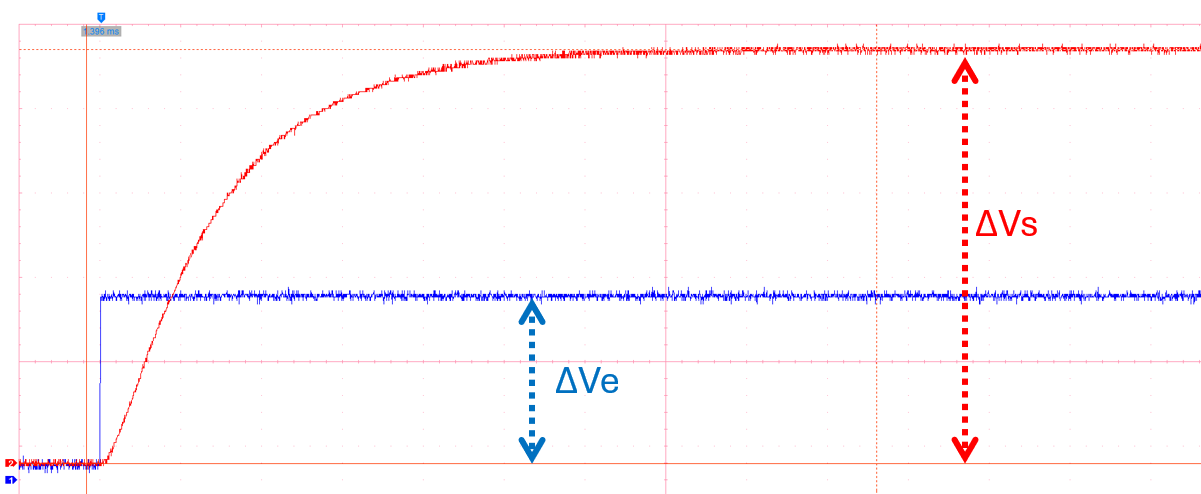
\includegraphics[width=0.5\textwidth]{images/ri_ordre1_out.png}
	
	%Cas d'un système passe-bas d'ordre 1 - mesure de la tension de sortie.
	
    \caption{Capture d'écran d'oscilloscope d'un échelon de tension $V_E$ (en bleu) appliqué à un système de type passe-bas d'ordre 1. La tension de sortie $V_S$ (en rouge) représente la réponse indicielle de ce système. Le calibre vertical est de 1V/carreau pour $V_E$ et de 1V/carreau pour $V_S$. L'échelle horizontale est de 1ms/carreau.}
    \label{fig:ordre1_gain}
\end{figure}



%%%%%%%%%%%%%%%%%%%%%%%%%%%%%%%%%%
\subsection{Mesure du temps de réponse}

Une autre information importante, en lien avec la bande-passante du système, est son temps de réponse. 

Dans le cas des systèmes d'ordre 1, le temps que met le système à atteindre 63\% de la valeur finale correspond à $\tau$, la constante de temps du système.

Dans la majorité des cas, on chercher à mesurer le temps que met le système à atteindre 95\% de sa valeur finale.

\medskip

La figure~\ref{fig:ordre1_response} montre une capture d'écran de l'acquisition à l'oscilloscope d'une réponse indicielle d'un système passe-bas du premier ordre.

Les positions de relevé de mesures des différents temps de réponse (63\% de la valeur finale pour un système d'ordre 1 ou 95\% de la valeur finale dans la majorité des cas) sont indiquées également sur cette figure.

\begin{figure}[h!]
    \centering
	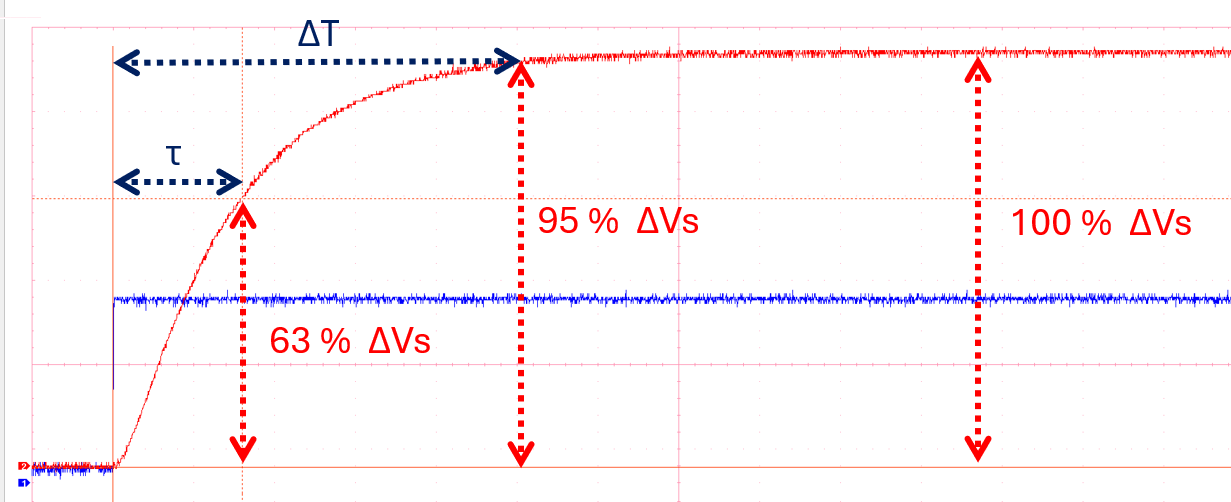
\includegraphics[width=0.6\textwidth]{images/ri_ordre1_out_63.png}
	
	%Cas d'un système passe-bas d'ordre 1 - mesures de la constante de temps et du temps de réponse à 95\%.
	
	    \caption{Capture d'écran d'oscilloscope d'un échelon de tension $V_E$ (en bleu) appliqué à un système de type passe-bas d'ordre 1. Mesures de la constante de temps et du temps de réponse à 95\%. La tension de sortie $V_S$ (en rouge) représente la réponse indicielle de ce système. Le calibre vertical est de 1V/carreau pour $V_E$ et de 2V/carreau pour $V_S$. L'échelle horizontale est de 1ms/carreau.}
    \label{fig:ordre1_response}
\end{figure}

\newpage
%%%%%%%%%%%%%%%%%%%%%%%%%%%%%%%%%%
\subsection{Autres mesures}

Il peut être intéressant de relever les valeurs des surtensions lors des \textbf{dépassements} (cas de systèmes d'ordre supérieur à 2). On peut par exemple, à l'aide des curseurs, mesurer le dépassement $D1$ (en lien avec le facteur de qualité d'un système du second ordre).

La période des oscillations $T$ peut également être mesurée (en lien avec la pulsation propre du système).

\medskip

La figure~\ref{fig:ordre2_dep} est une capture d'écran d'oscilloscope suite à l'acquisition d'une réponse indicielle d'un système passe-bas du second ordre. La méthode de mesure du premier dépassement ainsi que de la période des pseudo-oscillations est représentée.

\begin{figure}[h!]
    \centering
	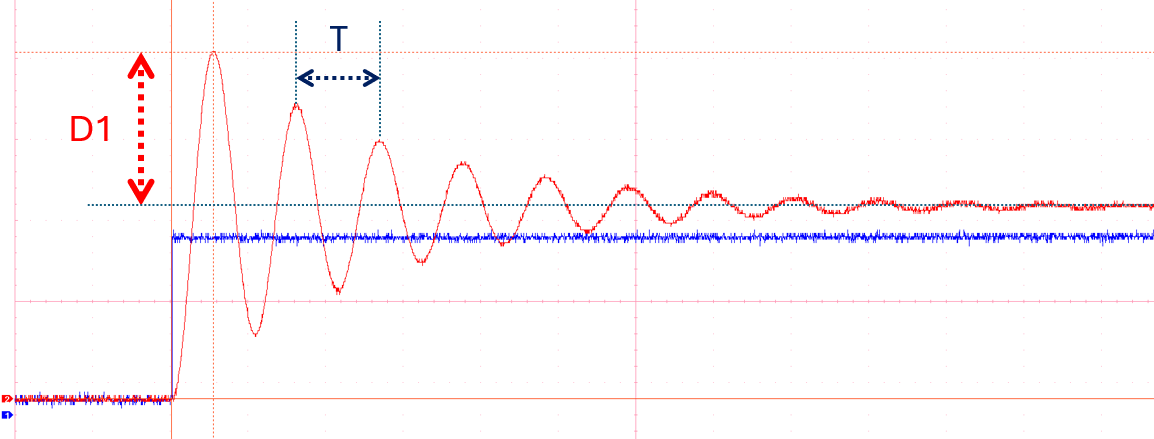
\includegraphics[width=0.6\textwidth]{images/ri_ordre2_bas_out_d1.png}
	
	%Cas d'un système passe-bas d'ordre 2 avec résonance - mesure de D1.    
	\caption{Capture d'écran d'oscilloscope d'un échelon de tension $V_E$ (en bleu) appliqué à un système de type passe-bas d'ordre 2 avec résonance. La tension de sortie $V_S$ (en rouge) représente la réponse indicielle de ce système. Le calibre vertical est de 1V/carreau pour $V_E$ et de 2V/carreau pour $V_S$. L'échelle horizontale est de 1ms/carreau.}
    \label{fig:ordre2_dep}
\end{figure}



%%%%%%%%%%%%%%%%%%%%%%%%%%%%%%%%%%
\subsection{Lien avec la réponse impulsionnelle et la réponse en fréquence}

La réponse indicielle est liée à la réponse impulsionnelle $h(t)$ d'un système par la relation suivante :

$$u_S(t) = \int_{0}^t h(x)dx$$

Cela signifie que la réponse indicielle est l'intégrale de la réponse impulsionnelle.

On rappelle également que la réponse en fréquence, que l'on peut modéliser par la fonction de transfert d'un circuit en fonction de la fréquence $H(j\omega)$ est la transformée de Fourier de la réponse impulsionnelle $h(t)$.